\documentclass{article}
\usepackage{cmap}
\usepackage[utf8]{inputenc}
\usepackage[english,ukrainian]{babel}
\usepackage{graphicx}
\usepackage{geometry}
\usepackage{listings}
\usepackage{float}
\usepackage{amsmath}
\usepackage{subfig}
\usepackage{xcolor}
\geometry{
	a4paper,
	left=20mm,
	right=20mm,
	top=15mm,
	bottom=15mm,
}
\lstset{
	tabsize=4,
	keepspaces,
	showstringspaces=false,
	escapeinside={(*@}{@*)},
	breaklines,
}
\graphicspath{ {./pictures} }
\setlength{\parindent}{4em}

\newcommand\subject{Архітектура комп'ютера}
\newcommand\lecturer{доцент кафедри ПЗ\\Крук О.Г.}
\newcommand\teacher{доцент кафедри ПЗ\\Крук О.Г.}
\newcommand\mygroup{ПЗ-22}
\newcommand\lab{8}
\newcommand\theme{Використання функцій BIOS для роботи з відео в текстовому та графічному режимах}
\newcommand\purpose{Опанувати функції BIOS для роботи з відео в текстовому та графічному режимах; розвинути навики складання програм для виведення різнокольорових рядків символів та графічних зображень; відтранслювати і виконати в режимі відлагодження програми, складені відповідно до свого варіанту}

\begin{document}
	\begin{normalsize}
		\begin{titlepage}
			\thispagestyle{empty}
			\begin{center}
				\textbf{МІНІСТЕРСТВО ОСВІТИ І НАУКИ УКРАЇНИ\\
					НАЦІОНАЛЬНИЙ УНІВЕРСИТЕТ "ЛЬВІВСЬКА ПОЛІТЕХНІКА"}
			\end{center}
			\begin{flushright}
				\textbf{ІКНІ}\\
				Кафедра \textbf{ПЗ}
			\end{flushright}
			\vspace{200pt}
			\begin{center}
				\textbf{ЗВІТ}\\
				\vspace{10pt}
				до лабораторної роботи № \lab\\
				\textbf{на тему}: “\textit{\theme}”\\
				\textbf{з дисципліни}: “\subject”
			\end{center}
			\vspace{112pt}
			\begin{flushright}
				
				\textbf{Лектор}:\\
				\lecturer\\
				\vspace{28pt}
				\textbf{Виконав}:\\
				
				студент групи \mygroup\\
				Коваленко Д.М.\\
				\vspace{28pt}
				\textbf{Прийняв}:\\
				
				\teacher\\
				
				\vspace{28pt}
				«\rule{1cm}{0.15mm}» \rule{1.5cm}{0.15mm} 2022 р.\\
				$\sum$ = \rule{1cm}{0.15mm}……………\\
				
			\end{flushright}
			\vspace{\fill}
			\begin{center}
				\textbf{Львів — 2022}
			\end{center}
		\end{titlepage}
		
		\begin{description}
			\item[Тема.] \theme.
			\item[Мета.] \purpose.
		\end{description}
		
		\section*{Індивідуальне завдання}
		\begin{figure}[H]
			\centering
			\includegraphics[scale=0.7]{v}
		\end{figure}
		
		\section*{Хід роботи}
		\subsection*{Код програми 1}
		\begin{lstlisting}[language={[x86masm]Assembler}]
INCLUDE C:/Irvine16.inc
.DATA

text1 BYTE 'K',118,'o',22,'v',76,'a',136,'l',213,'e',166,'n',36,'k',65,'o',87
text2 BYTE 'D',227,'m',26,'y',108,'t',27,'r',42,'o',150
text3 BYTE 'M',142,'y',91,'k',220,'h',207,'a',91,'i',241,'l',84,'o',175,'v',45,'y',248,'c',100,'h',35

.CODE
main PROC
mov ax,03h
int 10h

mov ax, SEG text1
mov es, ax
mov ah, 13h
mov al, 2
mov bh, 0
mov cx, (SIZEOF text1) / 2
mov dh, 8
mov dl, 30
mov bp, OFFSET text1
int 10h

mov ax, SEG text2
mov es, ax
mov ah, 13h
mov al, 2
mov bh, 0
mov cx, (SIZEOF text2) / 2
mov dh, 10
mov dl, 33
mov bp, OFFSET text2
int 10h

mov ax, SEG text3
mov es, ax
mov ah, 13h
mov al, 2
mov bh, 0
mov cx, (SIZEOF text3) / 2
mov dh, 14
mov dl, 38
mov bp, OFFSET text3
int 10h

RET
main ENDP 
END main
		\end{lstlisting}
		
		\begin{figure}[H]
			\centering
			\includegraphics[scale=0.7]{1}
			\caption{Результат виконання програми 1}
		\end{figure}
		
		\subsection*{Код програми 2}
\begin{lstlisting}[language={[x86masm]Assembler}]
INCLUDE C:/Irvine16.inc
.DATA

saveMode	BYTE	?
xVal		WORD	?
yVal		WORD	?

.CODE
main PROC

mov ah, 0Fh
int 10h
mov saveMode, al
mov ah, 0
mov al, 13h
int 10h
push 0A000h
pop es

mov dx, 3c8h
mov al, 1
out dx, al
mov dx, 3c9h
mov al, 0
out dx, al
mov al, 63
out dx, al
mov al, 0
out dx, al

mov xVal, 9
mov yVal, 12
mov ax, 320
mul yVal
add ax, xVAl
mov cx, 60
L1:		; 60 rows
	push cx
	mov cx, 90
	mov di, ax
	L2:		; 90 cols
		mov BYTE PTR es:[di], 1
		inc di
		loop L2
		inc yVal
		mov ax, 320
		mul yVal
		add ax, xVAl
		mov di, ax
		pop cx
		loop L1

	RET
main ENDP 
END main
\end{lstlisting}

\begin{figure}[H]
	\centering
	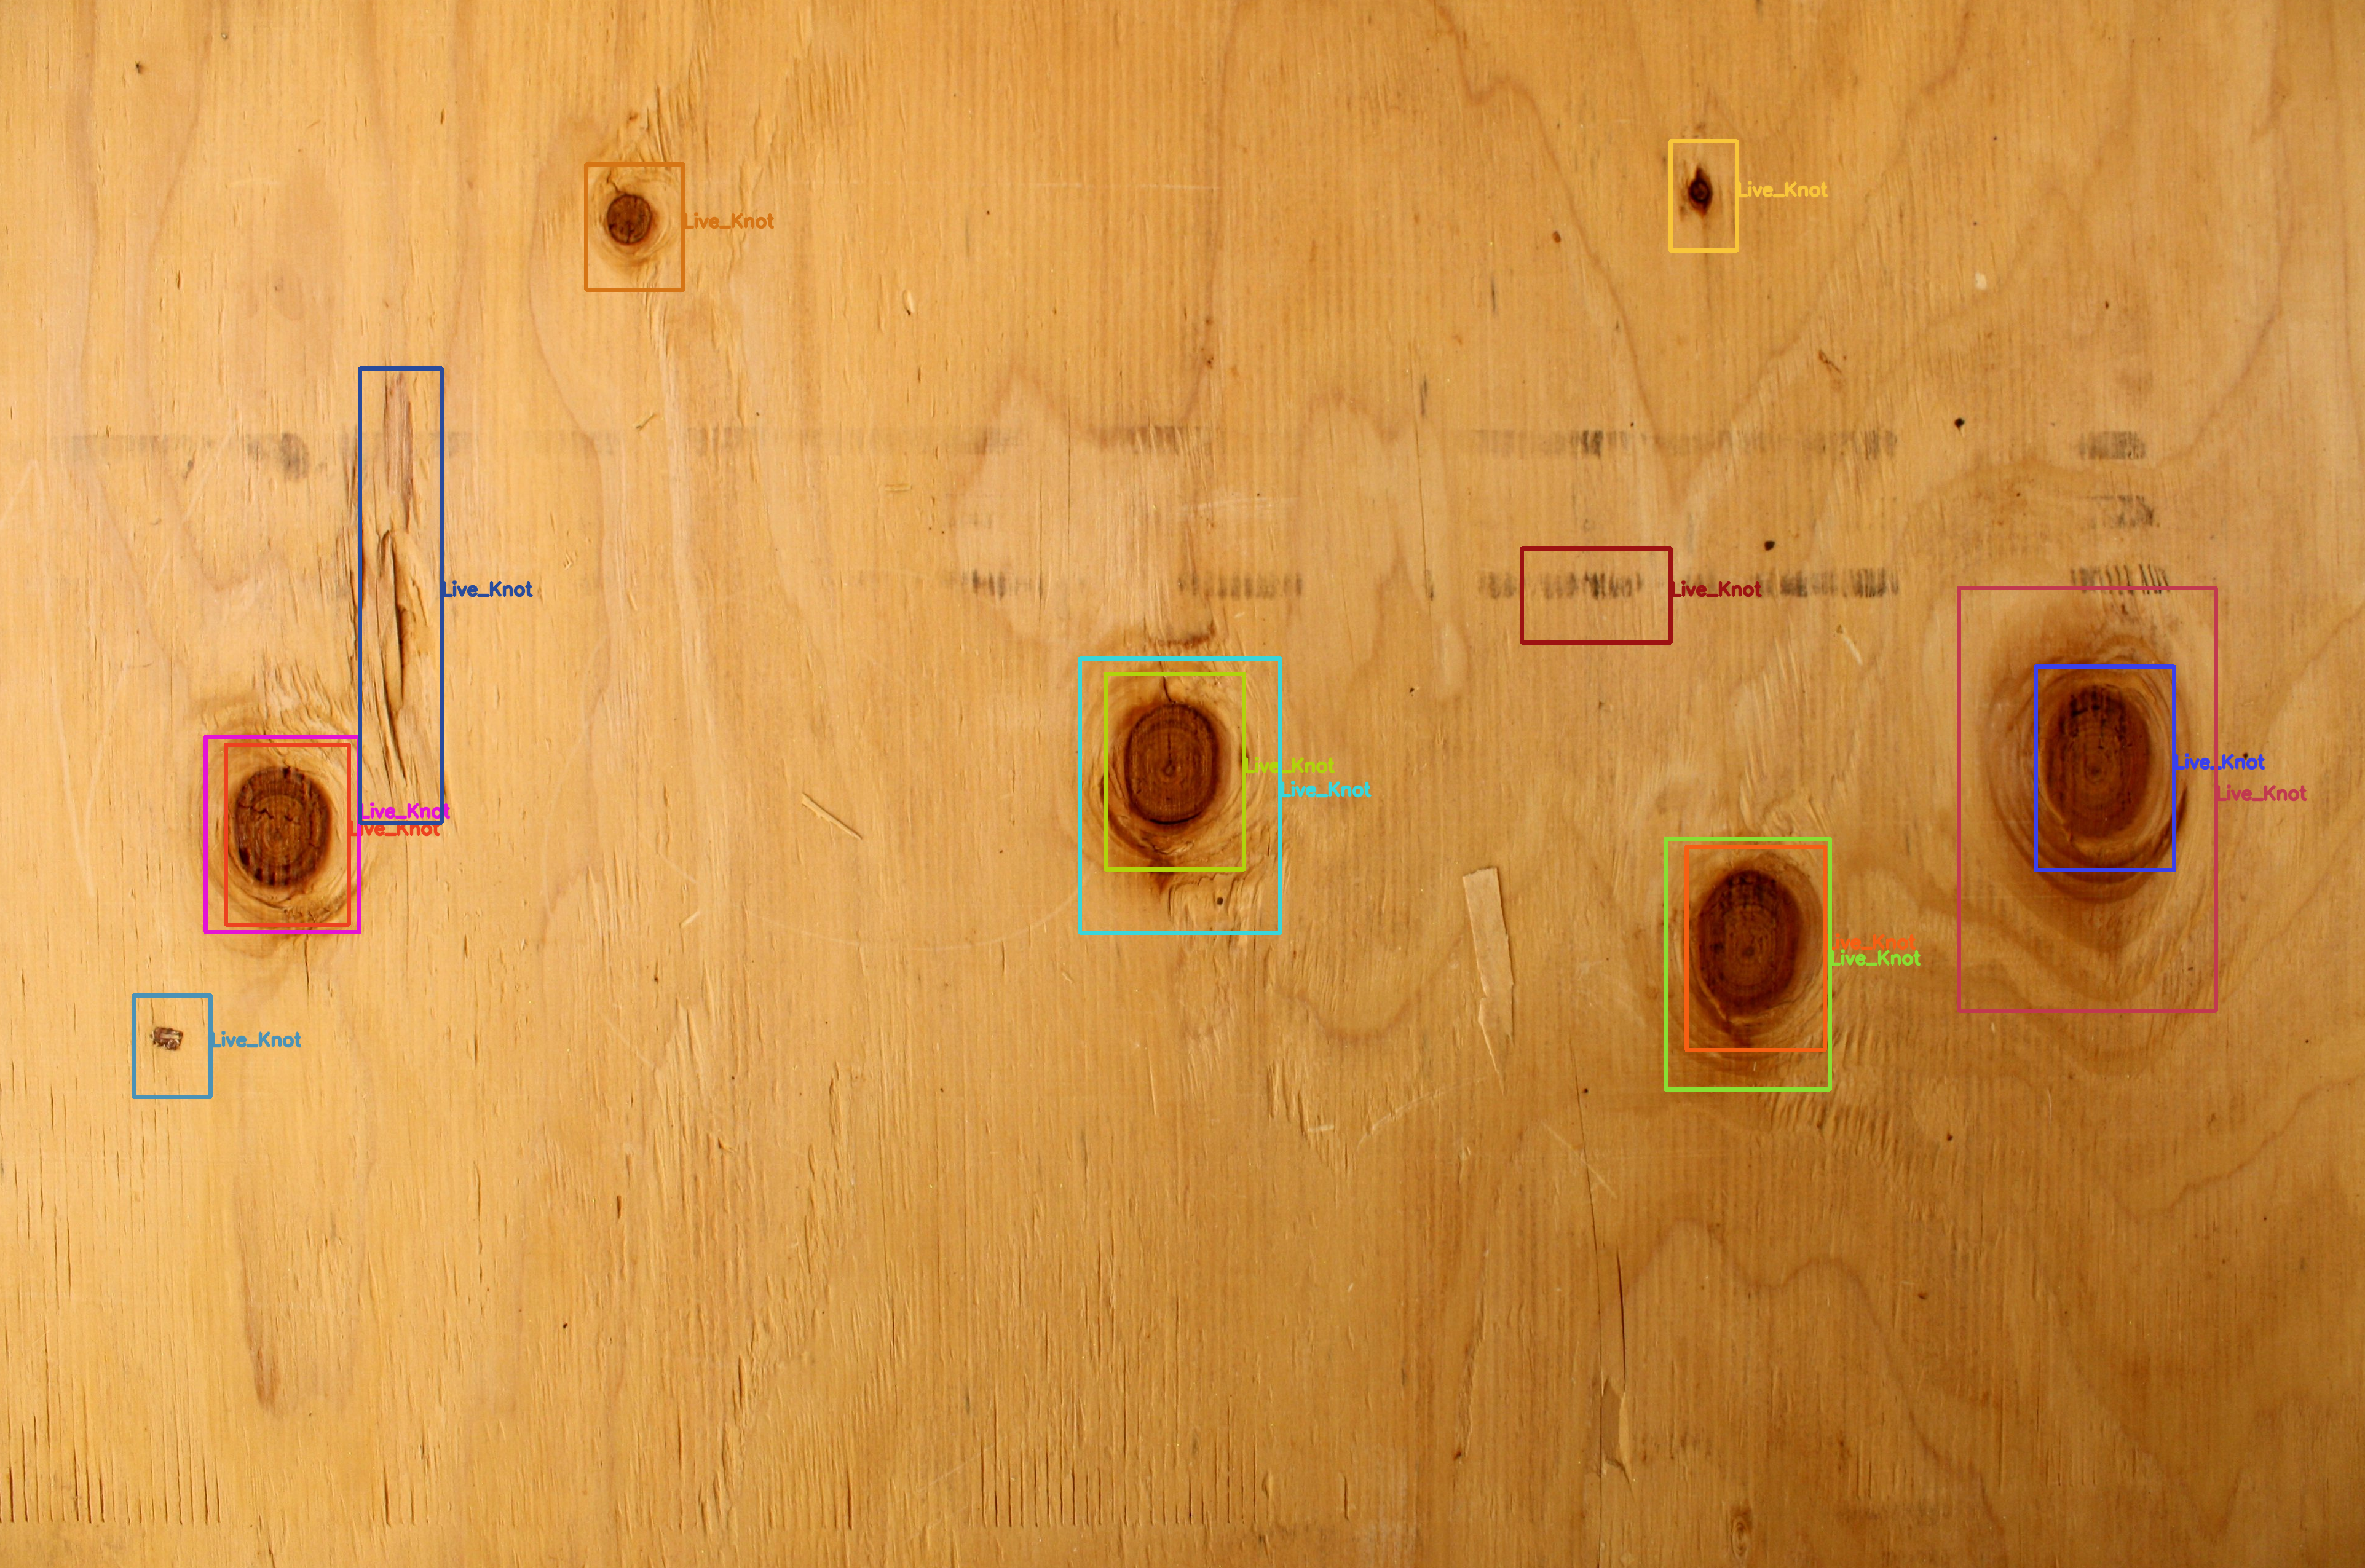
\includegraphics[scale=0.7]{3}
	\caption{Результат виконання програми 2}
\end{figure}
		
		\section*{Висновки}
		Під час виконання лабораторної роботи я опанував функції BIOS для роботи з відео в текстовому та графічному режимах; розвинув навики складання програм для виведення різнокольорових рядків символів та графічних зображень; відтранслював і виконав в режимі відлагодження програми, складені відповідно до свого варіанту.
		
	\end{normalsize}
\end{document}